%%%%%%%%%%%%%%%%%%%%%%%%%%%%%%%%%%%%%%%%%
% Academic Title Page
% LaTeX Template
% Version 2.0 (17/7/17)
%
% This template was downloaded from:
% http://www.LaTeXTemplates.com
%
% Original author:
% WikiBooks (LaTeX - Title Creation) with modifications by:
% Vel (vel@latextemplates.com)
%
% License:
% CC BY-NC-SA 3.0 (http://creativecommons.org/licenses/by-nc-sa/3.0/)
% 
% Instructions for using this template:
% This title page is capable of being compiled as is. This is not useful for 
% including it in another document. To do this, you have two options: 
%
% 1) Copy/paste everything between \begin{document} and \end{document} 
% starting at \begin{titlepage} and paste this into another LaTeX file where you 
% want your title page.
% OR
% 2) Remove everything outside the \begin{titlepage} and \end{titlepage}, rename
% this file and move it to the same directory as the LaTeX file you wish to add it to. 
% Then add \input{./<new filename>.tex} to your LaTeX file where you want your
% title page.
%
%%%%%%%%%%%%%%%%%%%%%%%%%%%%%%%%%%%%%%%%%

%----------------------------------------------------------------------------------------
%	PACKAGES AND OTHER DOCUMENT CONFIGURATIONS
%----------------------------------------------------------------------------------------

\documentclass[11pt]{article}

\usepackage[utf8]{inputenc} % Required for inputting international characters
\usepackage[T1]{fontenc} % Output font encoding for international characters
\usepackage{graphicx}
\usepackage{mathpazo} % Palatino font
\usepackage[legalpaper,margin=0.9in] {geometry}
\usepackage{fancyhdr}
\usepackage{float}

\setcounter{tocdepth}{4}
\setcounter{secnumdepth}{4}


\pagestyle{fancy}
\fancyhf{}
\lhead{\textsc{University of Regina}}
\rhead{\textsc{Software Systems Engineering}}
\cfoot{\thepage}

\begin{document}

%----------------------------------------------------------------------------------------
%	TITLE PAGE
%----------------------------------------------------------------------------------------

\begin{titlepage} % Suppresses displaying the page number on the title page and the subsequent page counts as page 1
	\newcommand{\HRule}{\rule{\linewidth}{0.5mm}} % Defines a new command for horizontal lines, change thickness here
	
	\center % Centre everything on the page
	
	%------------------------------------------------
	%	Headings
	%------------------------------------------------
	
	\textsc{\Huge University of Regina}\\[1.5cm] % Main heading such as the name of your university/college

	\textsc{\Large ENSE 477: Software Capstone Project}\\[0.5cm]
	
	\textsc{\Large Software Systems Engineering}\\[0.5cm] % Major heading such as course name
	
	
	
	
	%------------------------------------------------
	%	Title
	%------------------------------------------------
	
	\HRule\\[0.4cm]
	
	{\Huge\bfseries Workshop Enterprise Resource Planning Suite Requirements and Specifications Document}\\[0.4cm] % Title of your document
	
	\HRule\\[1.5cm]
	
	%------------------------------------------------
	%	Author(s)
	%------------------------------------------------
	
	\begin{minipage}[t]{0.4\textwidth}
		\begin{flushleft}
			\large
			\textsc{Authors}\\
			Jonathan Wells\\
			\textsc{200328640}\\ % Your name
			\large
			Konstantin Kharitonov\\
			\textsc{200354502} % Supervisor's name
		\end{flushleft}
		
	\end{minipage}
	~
	\begin{minipage}[t]{0.4\textwidth}
		\begin{flushright}
			\large
			\textsc{Supervisor}\\ % Supervisor's name
			Karim Naqvi\\
			M.A.Sc., P.Eng.\\
		\end{flushright}
	\end{minipage}
	
	% If you don't want a supervisor, uncomment the two lines below and comment the code above
	%{\large\textit{Author}}\\
	%John \textsc{Smith} % Your name
	%------------------------------------------------
	%	Logo
	%------------------------------------------------
	
	\vfill\vfill\vfill\vfill
	
\includegraphics[width=0.7\textwidth]{UR.png}\\[2cm] % Include a department/university logo - this will require the graphicx package
	 

	%------------------------------------------------
	%	Date
	%------------------------------------------------
	
	\vfill\vfill\vfill % Position the date 3/4 down the remaining page
	
	{\large\today} % Date, change the \today to a set date if you want to be precise
	
	%----------------------------------------------------------------------------------------
	
	\vfill % Push the date up 1/4 of the remaining page
	
\end{titlepage}

%----------------------------------------------------------------------------------------

%----------------------------------------------------------------------------------------
%Table of Contents %

\newpage 
\tableofcontents
%-------------------------------------------------------------------------------------

%-------------------------------------------------------------------------------------
%Table of Figures % 
\newpage
\listoffigures

%-------------------------------------------------------------------------------------
%Introduction%
\newpage
\section{Introduction}
The Workshop Enterprise Resource Planning Suite, or ERP for short, is an administrative task management web application primarily designed for the Engineering Workshop at University of Regina main campus. It is to be the main application to be used for managing incoming workorders, which are student and faculty submitted forms requesting the service of the shop. The service provides workorder capacity planning, allowing for the user to actively manage the status of each project, time tracking features for large scale and small scale work, as well as the ability to track the inventory of the workshop, including but not limited to, materials, tools and equipment. 
\subsection{Purpose}
This system was designed to replace the previous methods of workorder, time, and inventory tracking, centralizing all aspects into one powerful application that can be accessed online. Workorders currently must be submitted via paper form directly to the workshop during its operating hours. The form must then be reviewed by the workshop manager and if accepted, future meetings are scheduled. All workorders submitted are then stored physically in binders, which date back to the opening of the workshop. All materials and inventory are also stored physically. This project intends to automate all workorders and have then be submitted and archived electronically. As well, the system is intended to track all scopes of projects, ranging from small miscellaneous tasks to larger scale projects in such a fashion that the workshop manager can schedule them effectively in advance. 
\subsection{Scope}
ERP is designed as a Web API, such that it is run in browser and is able to be accessed from any computer with a sufficient internet connection. It will be a local application that will be primarily accessed by the workshop manager, who is this project's main client. Secondary clients include faculty and staff that wish to submit workorders over the ERP suite. The primary client is the only one intended to have full control of all features of the ERP suite. 
\newline
{\setlength{\parindent}{0cm}

The ERP Suite currently is planned to be exclusive to the engineering workshop based on its design as of the completion of this capstone project, as future work on this project will require a redesign to be re-purposed for future clients. The ideal future client for this program is for machine and workshop owners with a staff less than 50.  

\newpage

\section{Overall Description}
\subsection{Product Perspective}
The Workshop ERP suite is broken up into its 3 main functionalities: 

	\begin{enumerate}
	\item Workorders
	\item Time Tracking and Project Management 
	\item Inventory
	\end{enumerate}

Each feature can be accessed from the navigation side bar, which is present on all pages of the web application. 

\subsubsection{Workorders:}
On the workorder page, the client is able to access all workorders currently present in the system, whether they be first or historical submissions. Options include but not limited to, viewing user submissions, filter through all workorders, and tag them based on progress status and importance. The following figure showcases the different stages of a workorder throughout the submission process.
 
\begin{figure}[h]
	\centering
	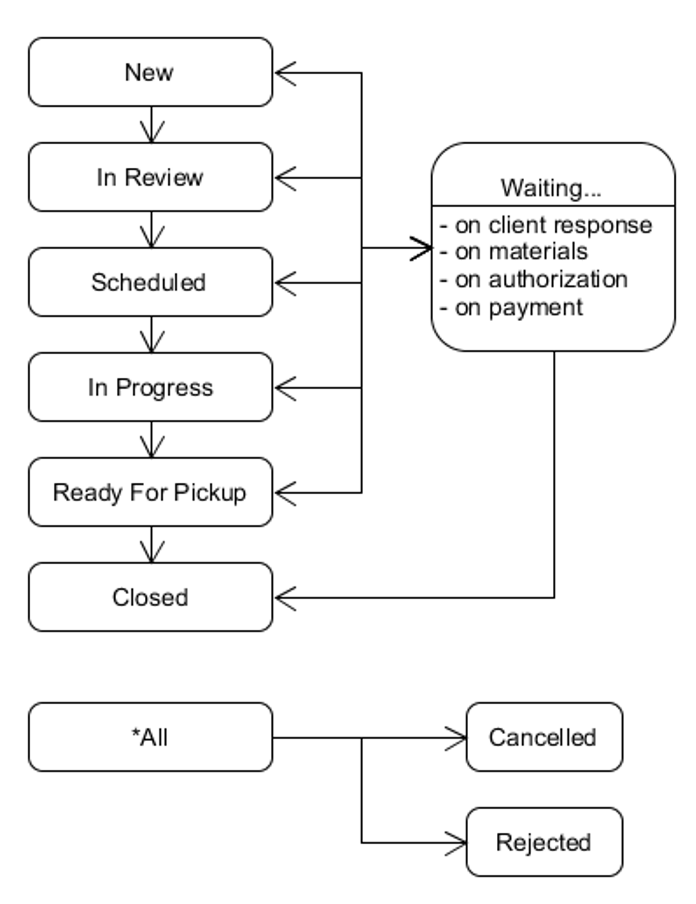
\includegraphics[width=5in]{workorder-status.png}\\
	\caption{Different Stages of a Workorder}
	\label{fig:tobias}
\end{figure}

\subsubsection{Time Tracking and Project Management:}
This page includes all of the time tracking features such as submitting current activities/projects into the system's calendar and creating a plan for workorders to be completed in the future. The time tracking page is also used for an accurate description of each semester, highlighting which project was worked each day. Functionality from this feature is also shown on the right navigation bar, allowing for quick access to daily tasks and which project deadlines are approaching the current date.

\subsubsection{Inventory:}
The inventory page is where the client is able to access and filter through the materials that are currently or previous were in stock in the workshop. Each material is able to be found inside the inventory database, as well as describing each based on filters such as type, amount, and length. Vendor information from where the material was purchased from and price per pound is also accessed from here. 

\subsection{Constraints}
As currently designed, the program is intended to only be used on campus. It is specific to the engineering workshop on campus and must go through a redesign before it can be distributed to a different client. As well, a steady internet connection is required to access the application as well as connect to the server hosting the application and its associated databases. The service is not optimised to mobile and as such, the user is heavily encouraged to the desktop version, though it is not a complete necessity. The program, from the perspective of the workshop manager, is not optimized for mobile use in its current stage.
\newline
{\setlength{\parindent}{0cm}

Some non-technical restraints include the application being unilingual to English, must be follow university guidelines of conduct, and requires a basic understanding of computing.  

\subsection{Operating Environment}
 The project is split into two main categories for development; the frontend and the backend. 
\newline
{\setlength{\parindent}{0cm}

On the front end, the client, who has the most control over the entire application. When the client log into the system upon start up, they have access to the main page displaying all necessary data for the particular day. In progress workorders, upcoming meetings and other related data can be quickly viewed. Clicking on a particular issue will navigate to a more in detailed view of the project. On the left side bar, the client can then access each particular section. 
\newline
{\setlength{\parindent}{0cm}

The first section is the Workorders page, where all workorders stored in the database can be accessed. Search and filtering options are available for the client when trying to locate specifics. Each workorder, displayed in a table with all necessary information, can be viewed, edited or deleted. When viewed in a closer look, tat particular workorder page is loaded, displaying all relevant information, including reference id, materials currently associated in the order, and all dates that apply. 
\newline
{\setlength{\parindent}{0cm}

The second section accessible by the left navigational bar is the time tracking feature, where the workshop manager can access the full calendar view of every time entry into the system, whether it is billable and non-billable hours. 

\subsection{Dependencies}
For the ERP suite function to provide the most value to the client, all data submitted inside application must be accurate, as the system will only perform based on the data that is given to the system. Workorders are assumed to be submitted in the proper predefined format such that crucial data is not lost throughout the project's lifetime. If a redesign of the workorder format is needed, documentation of this change is highly recommended.
\newline
{\setlength{\parindent}{0cm}
 
As well, all materials submitted into the inventory page must be properly accounted for in shop as well as on site. The program will display the information that it will receive, and changes to any inventory should be recorded as is necessary. The system relies on the user to file inventory data frequently to be considered up to date. 
\newline
{\setlength{\parindent}{0cm}

Since this application is currently being  developed in Sasktachewan, the system will use Staskatchewan standard time and will not account for any daylight savings that may occur if the program is used elsewhere in the work.

\subsection{User Documentation}
If there are any questions or concerns about running the program in its current state, there will be a set of two readme documents attached with both major aspects of the project. The frontend readme will describe the necessary information in running the server for the frontend, including how to run a localhost version in a development enviroment for testing. The backend readme as the information regarding running the backend server locally for development.

\newpage 
\section{System Features}
Since this system aims to modernize the current format of recording workorders and materials, this has a high priority for the workshop. While still a small scale project, it has potential to be vital in day to day operations for the engineering workshop. 

\subsection{Product Features}
There are three main users that will have access to the suite: the workshop manager, who is the main client, the student or faculty member that submits a workorder, and university administrators, who oversee the engineering workshop and its financial services. 

\subsubsection{Client}
The workshop manager is the main client for the ERP suite, and as such, they have the most access to the program. After logging in with their main id and password, the client is first faced with the main page of the application. This page features a daily snapshot of what is scheduled to be done during the day, such as any newly submitted workorders, any workorders that are nearing deadlines, any new comments submitted from the engineering administrators, and other notifications. From here, the client can use the left navigation bar to select any specific section for more details. 
\newline
{\setlength{\parindent}{0cm}

The workorders section is the first page, and is the most active of the options. This is where all of the incoming and historical submissions be viewable in a table. The table, which has search and filter features, showcases each workorder with all necessary data such as the sequential id, description and date, each having the possibility of viewing and editing. When a workorder is viewed, the full details are displayed, including materials used in the workorder, dates based on when the order was submitted and when it is due, as well as any administrative or client comments attached to the workorder. Each submission will have a unique sequential id, tied to the year and semester that the workorder was submitted. From this section, the client is able to plan further meetings with the requester, document their progress, and plan for billable and non-billable work. 
\newline
{\setlength{\parindent}{0cm}

The second section for is the time tracking page, where the client is able to view the workshop's schedule, submit new time entries, and plan ahead future project work. The default view is a monthly calendar, which features to allow for weekly and daily viewings. Each entry is also tagged with a level of importance, which can range from small day fixes all the way to large scale workorders. Each tag will appear with each entry on the calendar. The client can also add time entries, which require a description and level of importance tag, as well as a tag regarding whether the time  is billable or non-billable. 
\newline
{\setlength{\parindent}{0cm}

The final main section is the inventory page, which is where the all of the material data is stored. As in the workorders page, materials are viewable through a searchable table, which data such as material type, category and price visible. Pricing will be based off of the last known price of the particular material as well as the date the material was last purchased, done as a reference to see whether or not it is worth purchasing the material from the particular vendor. Materials can be filtered by the columns, showcasing exactly what the client is searching for. 
\newline
{\setlength{\parindent}{0cm}

On the right hand side of the program, the user has a quick access bar, which is a small scale viewing of the time tracking page. The client can quickly scroll through day by day on any upcoming deadlines, submissions, and other meetings without having to leave from the current page. This page is viewable from each section within the application. 

\subsubsection{Administration}
For the university administration side, they are able to see the workorders submitted to the workshop as well as the comments that have been made on each order. The administration will have access to create their own comments, communicating towards the workshop manager. Administration is also able to view the time tracking session, seeing what is scheduled for the shop manager in much the same way as the manager can, but they do not have access to add, edit or delete any entry. 

\subsubsection{Student/Faculty}
The student or faculty member submitting a workorder will have a vastly different page that they will have access to. The submitter would log into the the page with an approved University of Regina account. Once logged in, the user will see a form for submitting a workorder. Here they will complete an order, filling out each section similar to the paper form that is used previous to the application. Once submitted, the user is prompted to send their email such that the workshop manager can have communication with the requester during the process. 
 
\section{External Integrations}
For this project, there are features that he application must have access to before it is able to be full functional. 

\subsection{Financial Services}
When a student or faculty member logs into the application and submits a workorder, their account must have access to their particular university financial account so that the workorder can be charged to it upon the competition. This will be done through financial services, and will require additional authentication using the financial account of the student or faculty member. Currently to create a workorder, the requester would use their Novell login information, as would on any other university application. 

\subsection{UR Internet}
The ERP suite must have a connection to the University of Regina's internet during runtime, so that the application's data can be updated and communication between the workshop manager, the requester and the administrators can be maintained. Without this connection, then no data can be loaded on to the application.  


\section{Non-Functional Requirements}

\subsection{Security Requirements}
For the system to stay secure and accurate, personal account data must be not be distributed without caution. the workshop manager should chose an account and password that is very secure and should refrain from sharing that information with others, including the University of Regina engineering administration and other faculty members. The connection to the database that holds the workshop's information should also be kept private, such that no data is tampered with. 

\subsection{Safety Requirements}
In the case of a crash in the system, or a crash in the database server, please refrain to an older version of the software. All versions can be found on our github page, included with all of the installation guides and other necessary documentation.

\section{References}


\end{document}


